% Chapter Template

\chapter{Examining finite-size effects in thermal conductivity computations} % Main chapter title

\label{Chapter3} % Change X to a consecutive number; for referencing this chapter elsewhere, use \ref{ChapterX}

%-----------------------------------------------------------
\section{\label{sec:3.intro}Introduction}
%-----------------------------------------------------------

!!! EDIT THIS - HOW MUCH OF THIS HAVE I EXPLAINED ALREADY? HOW MUCH IS THAT A PROBLEM?

Knowledge of the thermal conductivity of solids is key in a wide range of technological applications and for our understanding of natural systems. For example, in the Earth's lower mantle thermal conductivity controls the nature of planetary convection \citep{Tosi2013}, and the heat flux out of the core which powers the geotherm. Low thermal conductivities are required in thermoelectric materials, to maximise the efficiency of heat-electricity conversion \citep{Snyder2008}.

A range of atomic scale simulation methods are available to determine the lattice thermal conductivity of materials. These are invaluable for calculating thermal conductivity at conditions of which experiments are difficult, e.g. the extreme conditions found in the Earth's lower mantle (pressures and temperatures up to 136~GPa and 4000~K at the core-mantle boundary).

%(MOVE - to where though?) Many studies assume lowermost mantle thermal conductivity to be 10~\wmk~\citep[e.g.][]{Lay2008}, but uncertainty in the extrapolation of results made at low pressures and temperatures gives a range of 4~-~16 \wmk~\citep{Brown1986, Osako1991, Hofmeister1999, Goncharov2009, Manthilake2011, Ohta2012}.

%---------------------------------------
\subsection{\label{sec:3.FSE}Finite-size effects}
%---------------------------------------

!!! HOW MUCH OF THIS HAVE I EXPLAINED ALREADY? HOW MUCH IS THAT A PROBLEM?

As discussed previously, care must be taken to ensure simulations are faithful to the material and physical conditions. Perhaps most obvious is ensuring you are representing the chemistry correctly, that the atoms have correct charges, masses, and interactions with neighbours. Even if this chemical information is completely accurate, simulations can produce results wildly different to reality if you do not have enough atoms to reproduce the behaviour of the bulk material. In the case of thermal conductivity, this means ensuring phonons are behaving properly.

Conductivity will be underestimated if the length of the system is comparable to the dominant heat-transporting phonon wavelengths. Phonons that cannot be resolved in the system, cannot contribute to heat flow therein. Another way the effect of finite system size can be observed is in the reproduction, of failure thereof, of thermal resistance. Phonons scatter off of one another, impeding the flow of heat from one point to another. Assuming the above point of having enough length to support phonon wavelengths is considered, phonon-phonon scattering in the direction of heat flow will be accurate. What will not necessarily be correct is the ph-ph scattering in the directions perpendicular. The above principal applies, if the system has too small a cross-sectional area (compared to its length), the phonons involved in lateral scattering cannot be resolved. This tends to reduce thermal resistance within the system, thereby overestimating conductivity.

The severity of these finite-size effects (FSE) increases with the length and expected travel distance of phonons. Longer phonons require longer systems in which to resolve them. This means I want to investigate the conditions at which conductivity will be largest. This means low temperatures, high pressures, and no impurities. While the result of interest is the conductivity at the CMB, 136~GPa and 4000~K, I will also investigate the FSE at 136~GPa  and 1000~K, both considering chemically and isotopically pure \mgsios \bdg.



%-----------------------------------------------------------
\section{\label{sec:3.direct}Direct method}
%-----------------------------------------------------------

In this section I will talk specifically about how I apply the direct method to compute the \tcs of \bdg. I cover the initial system setup, the supercell geometry and how the system is divided into sections to determine the temperature gradient. I then cover properties which must be monitored to ensure accurate results, namely the magnitude of the temperature difference across the gradient, and the convergence of computed conductivity with total simulation time. I briefly introduce the data processing methodology, before explaining how the effects of finite system size are considered and mitigated. Finally I correlate my observed results with theoretical predictions, and discuss the required system size to compute the conductivity of \bdgs at lower mantle conditions.

!!! FLOW CHART, OVERVIEW FIGURE OF BELOW STEPS AND PROCESS?


%---------------------------------------
\subsection{\label{sec:3.DM.cell}Setting up supercells}
%---------------------------------------

!!! HOW IS HEAT FLOW ESTABLISHED? REF BACK? MULLER PLATHE

In order to investigate how FSE can affect direct method results, I plan to use very large cells, both in length and cross sectional area. To capture a large section of inverse-length space during processing (more on this later, REF?), I will use supercells up to 96 unit cells long in the x-direction of heat flow (specifically 6, 8, 10, 12, 16, 24, 48, and 96 unit cells long). Perpendicular to this length, I will use supercells with a cross section up to 12$\times$12 unit cells (1$\times$1, 2$\times$1, 2$\times$2, 4$\times$4, 8$\times$8, and 12$\times$12).

The simulation supercell is split into sections along its length, where the average temperature of atoms within is determined to calculate the gradient across the system. The symmetry of the \bdgs crystal system allows unit cells to divided into two, such that the width of sections is half a unit cell along the length of the supercell (the direction of heat flow). 

Two of these sections, half the supercell length apart, are designated as the heat source and heat sink. It is within these sections that the energy of the atoms is swapped. Heat flows in both directions from the hot section because of cell periodicity (refer back to Section \ref{sec:2.DM.setup}), meaning there are two temperature gradients to sample and combine. 

Where L is supercell length in unit cells and S (= 2L) gives the number of sections, we obtain S/2 + 1 temperature points to fit the gradient. Width of a section, S$_{\mathrm{W}}$, is half that of a single unit cell. Because the temperature gradient is non-linear around the heat source and sink, we ignore S/12 sections (rounded to nearest integer) from both ends of the temperature gradient. For a given simulation cell we fit S/3 + 1 points to obtain the temperature gradient. We use a minimum supercell length of 6 unit cells (12 sections, 5 data points), in order for sufficient fitting of the temperature gradient. 

%\begin{figure}[h!]
%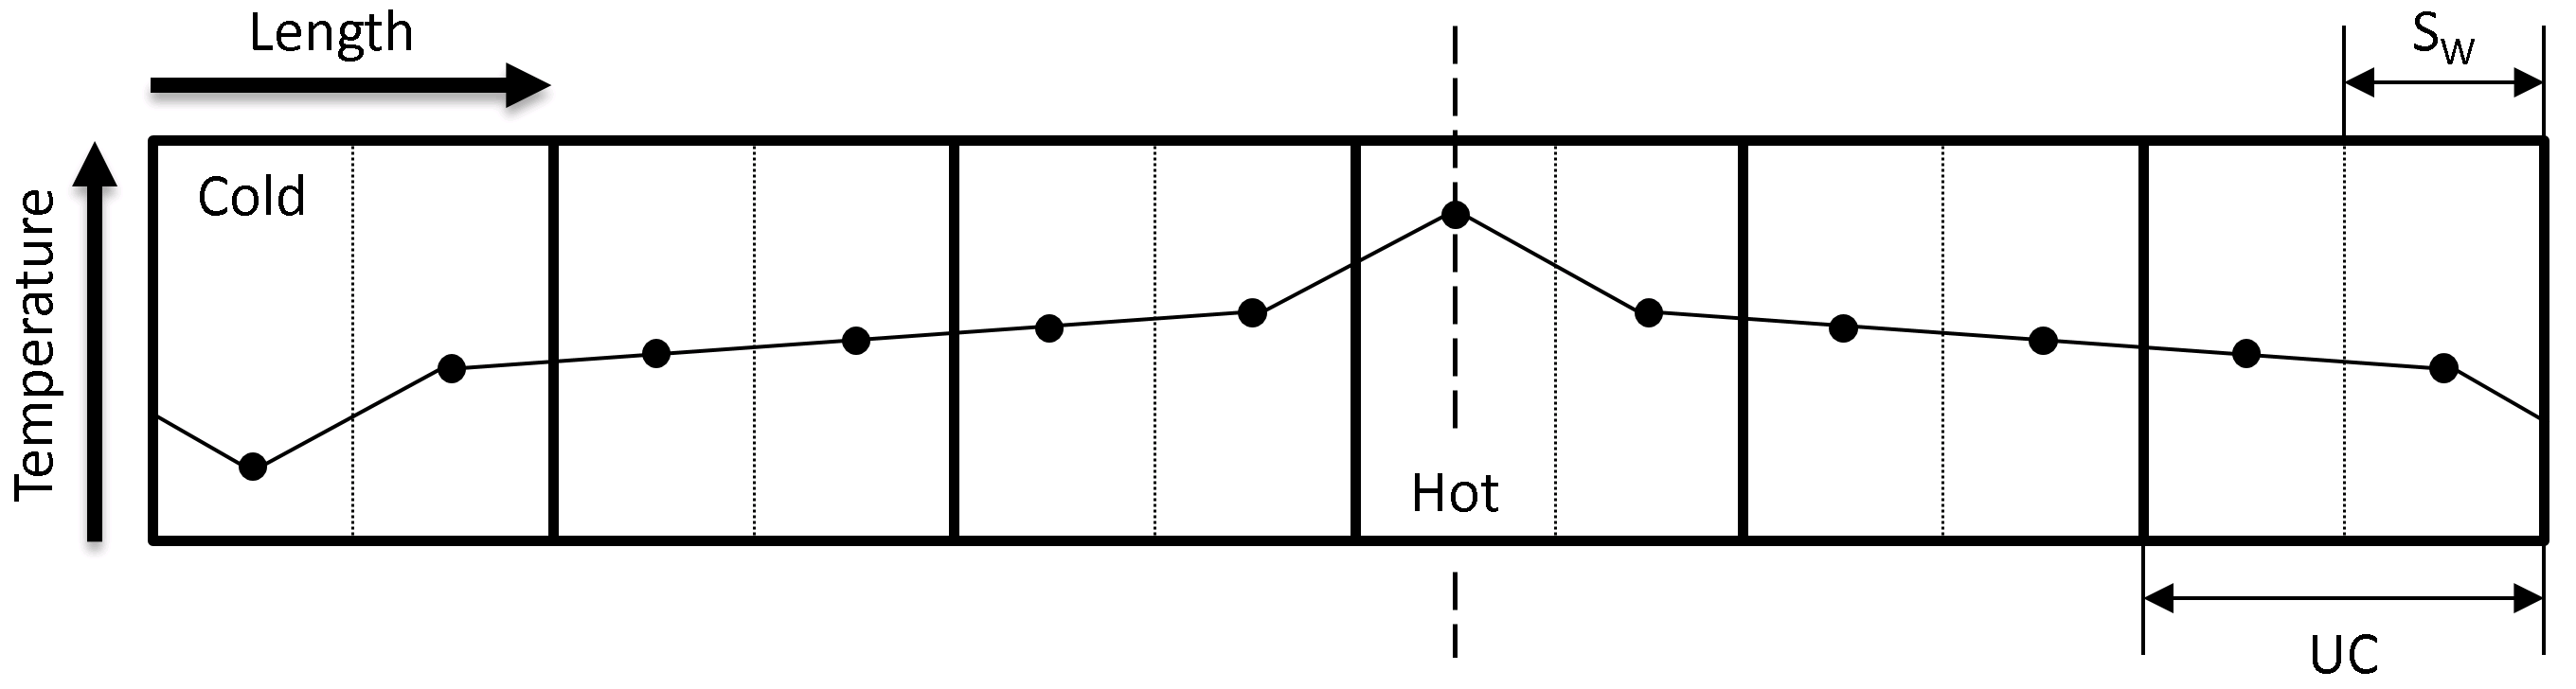
\includegraphics[width=\linewidth]{Figures/direct_temp_pro_01.png}
%\caption[direct temperature profile 1]{}
%\label{fig:direct_temp_pro_01}
%\end{figure}

%\begin{figure}[h!]
%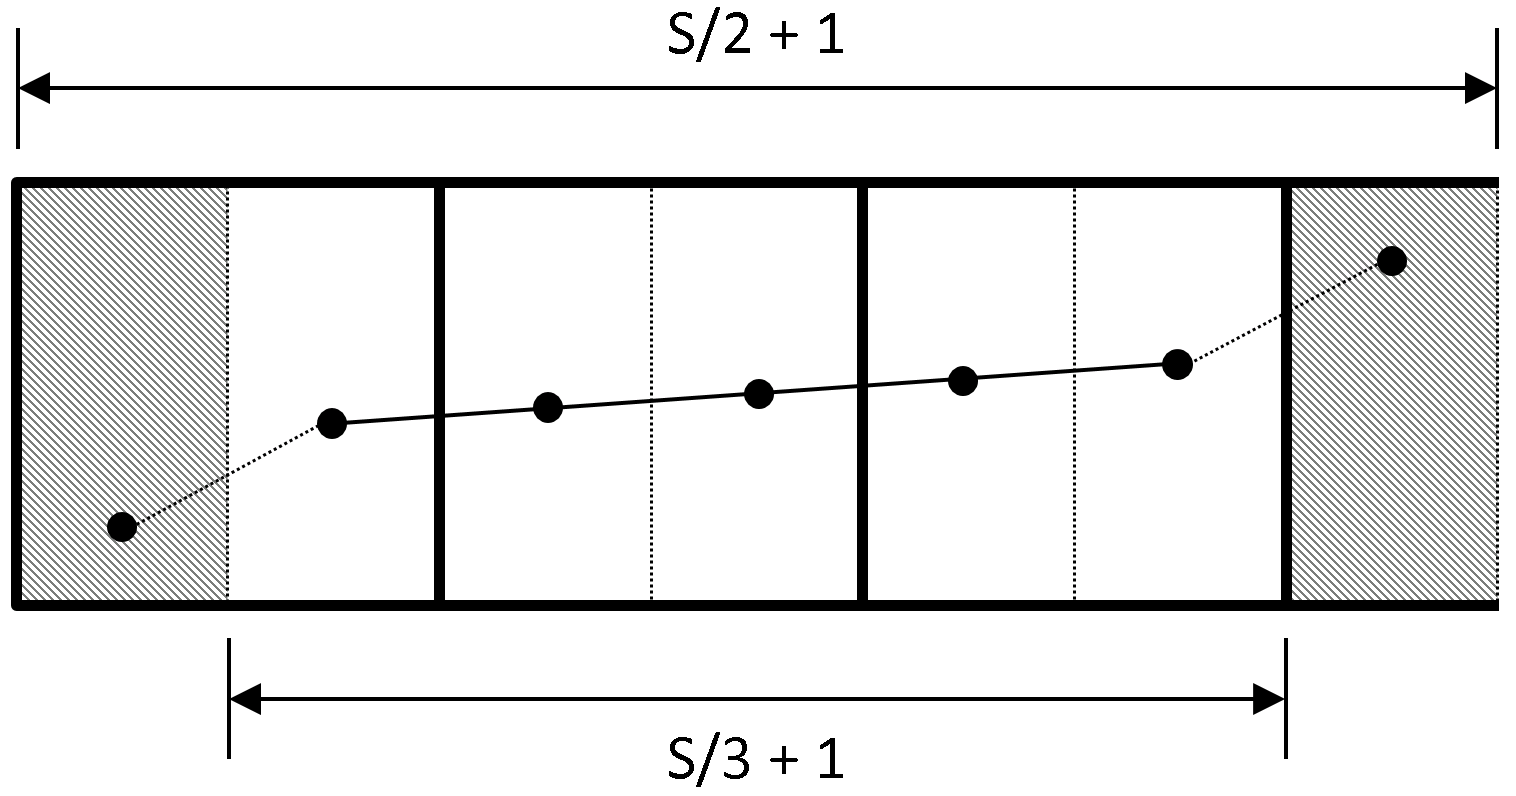
\includegraphics[width=\linewidth]{Figures/direct_temp_pro_02.png}
%\caption[direct temperature profile 2]{}
%\label{fig:direct_temp_pro_02}
%\end{figure}

\begin{figure}[h!]
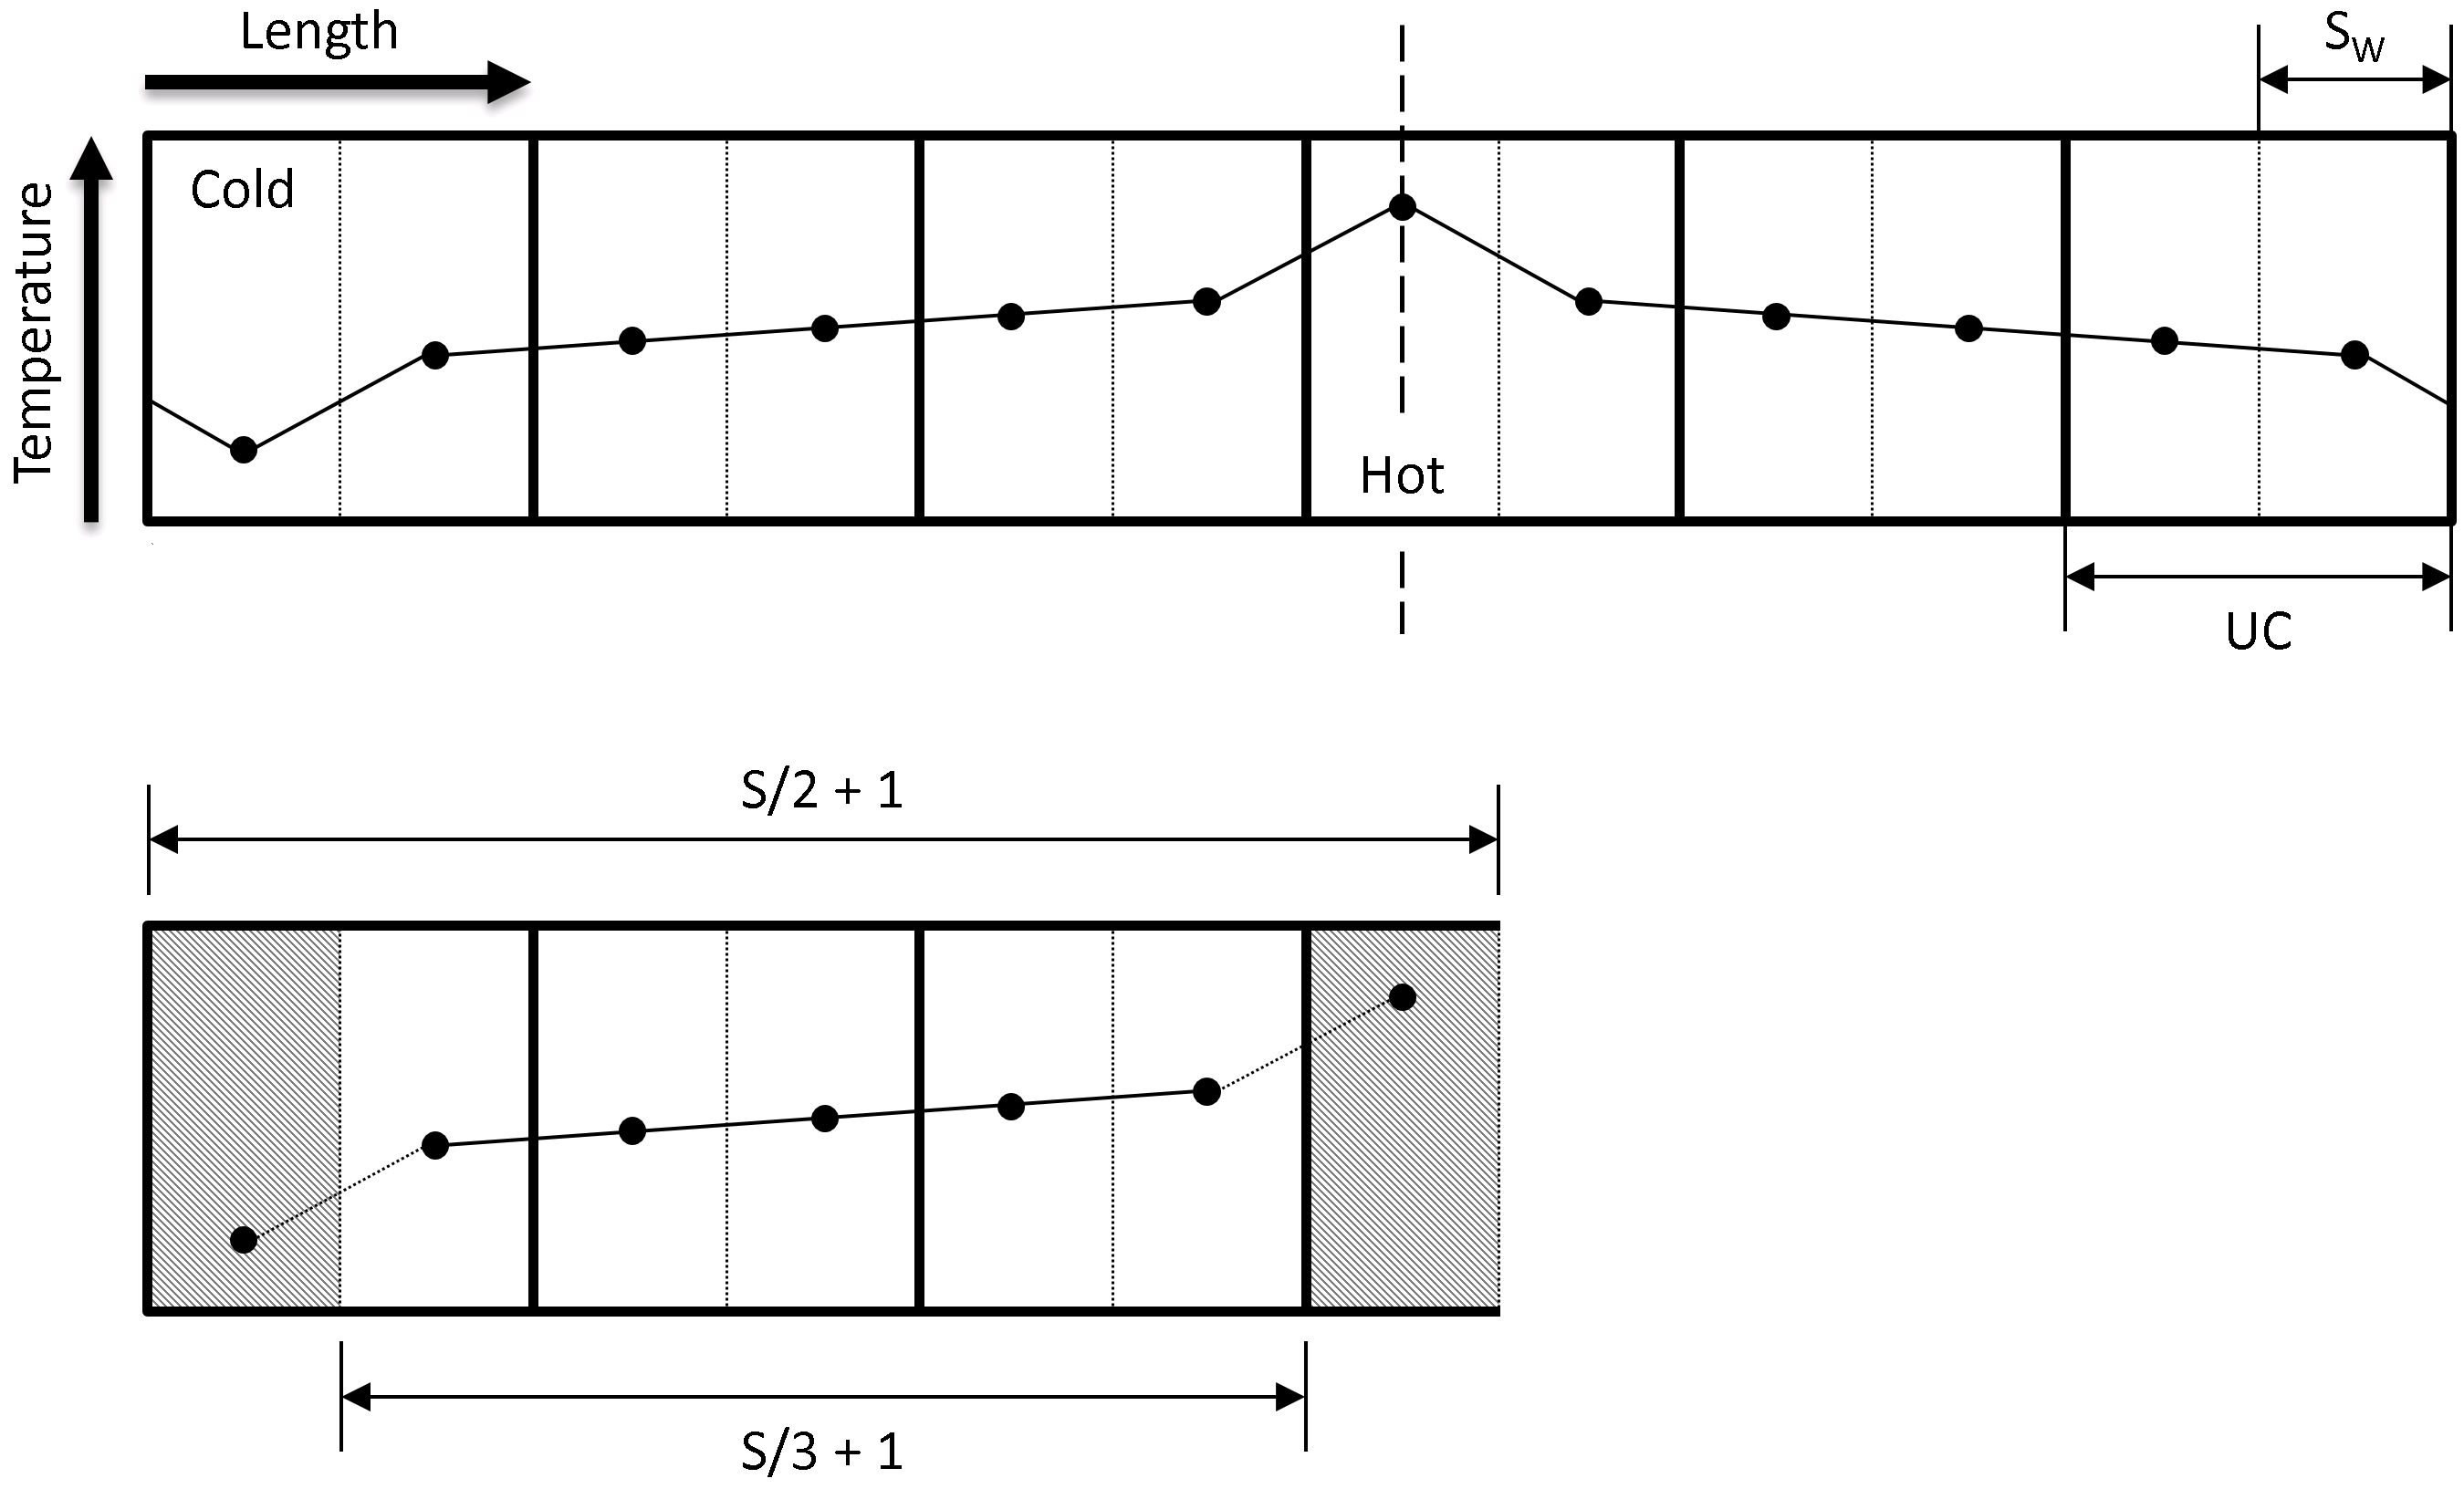
\includegraphics[width=\linewidth]{Figures/direct_temp_pro_03.png}
\caption[direct temperature profile 3]{}
\label{fig:direct_temp_pro_03}
\end{figure}

%---------------------------------------
\subsection{\label{sec:3.DM.bin}FIDDLING WITH BIN WIDTH}
%---------------------------------------

!!! DOES THIS SECTION NEED TO EXIST?

Changing the width of the heated sections has no effect on the conductivity result, assuming you have enough temperature points to fit the linear gradient. Furthermore, changing the width (and thus number) of temperature bins has no effect on the sampled gradient, assuming resolution is large enough to capture the non-linear region around the heat source/sink (see Figure~\ref{fig:direct bin width}). 

\begin{figure}[h!]
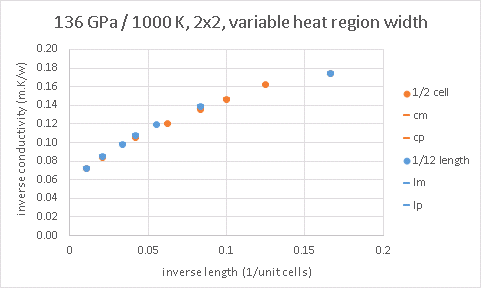
\includegraphics[width=\linewidth]{Figures/direct_bin_width.png}
\caption[direct bin width]{Conductivity results from direct method when temperature is calculated from sections half a unit cell wide, and also a twelfth of the total length. The amount of points in the temperature gradient changes when the section width depends on the unit cell, but not on the length (i.e. there are always twelve sections, the gradient is fit to five data points).}
\label{fig:direct_bin_width}
\end{figure}


%---------------------------------------
\subsection{\label{sec:3.DM.grad}Temperature gradient convergence}
%---------------------------------------

!!! GRAPHS AND STUFF - EDIT HEAVILY!

An important factor for utilising the direct method is maintaining a sensible temperature gradient, such that Fourier's law (REF) remains valid, i.e. conductivity is constant along the length of the cell. Thermal conductivity is strongly temperature-dependent at upper lower-mantle conditions (1000~K), it is therefore undesirable to have substanially different conductivities as a of function of temperature across the cell. The opposite case is also true, the difference in temperature between hot and cold sections must be larger than the uncertainty in the average system temperature. 

As a general rule, I try to keep the temperature difference between the ends of the gradient to 20\% the mean temperature. I control the magnitude of the gradient by altering the interval at which heat is exchanged, via swapping atomic velocities in the hot and cold sections (see Section \ref{sec:2.DM.setup}) . To produce the desired gradient magnitude as outlined above, shorter intervals are required as cell length decreases, cross-sectional area increases, and system equilibrium temperature decreases. The easier it is for heat to flow from hot to cold (smaller distance between, more area for heat transport, lower temperature/less thermal resistance), the more heat must be transported (in the form of shorter intervals between heat swaps) to maintain a temperature gradient.


%---------------------------------------
\subsection{\label{sec:3.DM.time}Simulation time convergence}
%---------------------------------------

!!! SHOW CONVERGENCE ONCE, THEN ASSUME READER HAS FAITH IN ME

Initial results from the direct method show a large variability in conductivity, despite the seperate temperature equilibration performed beforehand. This is related to the setup of the temperature gradient and its transition to steady behaviour. For this reason, the timesteps containing this behaviour are ignored when determining conductivity. This simply means removing the temperature gradient and heat flow data from the rest of the series. How this is applied varies in practice, but on a 1~ns simulation, I would typically ingnore the first 100~ps (10\% simulation time).

!!! FIGURES NEEDED EVERYWHERE

After removing the first portion of the data there is still variability in the calculated conductivity, but this typically converges quickly over the course of the simulation. If you have enough timesteps, the cumulative average of conductivity will tend towards a value while the uncertainty decreases. This is a simple check to ensure accurate results, where the simulation can be extended if more data is required.

!!! FIGURES NEEDED EVERYWHERE

It is possible for a simulation to be too long however, where the conductivity result will drift from its converged position. This is due to inaccuracies in the molecular dynamics calculations, typically in the form of steepening temperature gradient over time. It is difficult to spot by just looking at the conductivity result and uncertainty, but easy to observe in the time series and/or graphically. The conductivity value obviously begins to change irratically, and the uncertainty begins to increase. The uncertainty would never increase if the result was still converging, making this a useful marker to look for in the series.

!!! FIGURES NEEDED EVERYWHERE


%---------------------------------------
\subsection{\label{sec:3.DM.data}Data processing}
%---------------------------------------

!!! FLYVBERG AND STUFF - ASK STEPHEN


%---------------------------------------
\subsection{\label{sec:3.DM.extrap}Inverse extrapolation procedure}
%---------------------------------------

!!! SCHELLING, EXPLAIN IF I DIDN'T EARLIER


%---------------------------------------
\subsection{\label{sec:3.DM.fse}Finite-size effects}
%---------------------------------------

!!! HEAVY REWORK NEEDED - FIGURES EVERYWHERE

OBVIOUS CSA - One thing that is immediately obvious is that supercell CSAs of 1\by1 and 2\by1 overestimate conductivity (underestimate inverse conductivity) with respect to the larger CSA. As discussed earlier, this can attributed to the absence of realistic phonon scattering within a narrow material. For the supercells with shorter lengths (larger inverse length), increasing CSA (to 2\by2) brings the results into alignment. 

TOO SHORT - Another problem becomes apparent when looking at the 1000~K results, the shortest cells in the series (longest inverse length) appear to overestimate conductivity (underestimate inverse etc.) with respect to the expected linear fit through the other short cells. This can be explained by the cell being on the order of the phonon MFP, allowing for phonons to travel from hot to cold without any scattering events (Ballistic Phonon Transport). This means the simulation does not have thermal resistance representative of the material. No correction can be applied here, the 6 unit cells long cells must be excluded from the extrapolation. The problem does not seem to be present in the 4000~K results, the explanation being that the unit cell is larger from thermal expansion, and more significantly, the phonon MFP is shorter with higher temperature.

!!! MFP ANALYSIS?

NOT-OBVIOUS CSA - Lorem Ipsum
















%---------------------------------------
\subsection{\label{sec:3.DM.theory}Explaining CSA effect}
%---------------------------------------

!!! GO THROUGH THEORY WITH STEPHEN


 










%-----------------------------------------------------------
\section{\label{sec:3.GK}Green-Kubo}
%-----------------------------------------------------------

!!! DO I NEED TO MENTION HOW TO PERFORM ACF IN C2?

Now I will outline my approach for applying the Green-Kubo method for computing conductivity to \bdgs at lower mantle conditions. First I show accurate results can be obtained within the chosen correlation length. I then show how results represent a large sample of possible conditions, and a way of minimising error by combining multiple heat flux autocorrelation functions (ACFs). Finally I show that all these components are valid with respect to total simulation time, before presenting how finite simulation size affects conductivity results.

After determining cell parameters appropriate to the simulated conditions (NPT), I initialise a temperature distribution (NVT). To obtain heat flux auto-correlation functions, a simulation for each initial temperature condition is run for X~ns, with 9 successive repeats for a total of 10 jobs. This gives 10 ACFs from each initial condition. Simulation runs are split in this manner to be feasible computationally, jobs submitted to the high-performance computing facilities have a maximum length of 48~hours. Each job finished in this manner produces an ACF, somewhat of a bootstrapping process on the total simulation series.

%---------------------------------------
\subsection{\label{sec:3.GK.cor}Correlation length convergence}
%---------------------------------------

!!! Show high and low temperature, difference in start and end of correlation window.

In this study we compute ACFs up to correlation lengths of 100~ps, with (100,000) 1~fs timesteps. This length is longer than required but selected as a proof of concept to show convergence in the conductivity result, additionally to display the extent and behaviour of drift in the integrals for long correlation times. We show in Figure \ref{fig:acf_decay} that the magnitude of the ACF decays to much less than 1\% of its initial value around a correlation time of 2~ps, inferring the start of convergence for the integral and thus conductivity.

!!! INSERT FIGURES HERE

Considering bridgemanite at lower mantle conditions, we find correlation time windows in the range of 2-30~ps to be suitable. At the low-end, this allows the initial high-variability in integral value to be ignored. At the high-end, the time is long enough for good sampling of the integral, but short enough to ignore the drift-effects. The magnitude and range of the window typically increases with conductivity (or with decreasing temperature etc.), e.g. 2-10~ps at 4000~K, and 10-30~ps at 1000~K. These correlation lengths are on the same order of magnitude as used by \citet{Haigis2012}. They observe convergence in the conductivity result after 30~ps, albeit at a temperature of 300~K. This corresponds with what I noticed, lower temperatures/higher conductivities require longer ACF.

%---------------------------------------
\subsection{\label{sec:3.GK.int}Integral sample convergence}
%---------------------------------------

!!! Is this section even necessary? Bootstrap the integrals, show result doesn't change?

ACFs produced by each simulation are integrated seperately, and averaged into a single series. 
%This process is performed for heat fluxes in each crystallographic direction, to allow analysis of anisotropy and finite system size effects.  
From this combined integral we pick a window of correlation lengths to capture a flat, converged region (or the section just after the 'bottleneck' if convergence is not obvious). This correlation length window is then applied to all integrals constituent to the combined series, giving a sample of integral averages and corresponding standard deviations. A weighted average is then taken of these data points, to give a single value with uncertainty. This value is directly proportional to thermal conductivity, as given by Equation \ref{gk-int}. REFERENCING TOO FAR BACK? REPEAT EQUATION?

%---------------------------------------
\subsection{\label{sec:3.GK.sim}Simulation length convergence}
%---------------------------------------

%!!! SIMULATION LENGTH CONVERGENCE BY FIDDLING WITH profile.heatflux AND pull_list.bash

%!!! HAIGIS RUN FOR AT LEAST 0.5NS - SIMULATION LENGTH CONVERGENCE OTHER WORKS

%---------------------------------------
\subsection{\label{sec:3.GK.fse}Finite-size effect convergence}
%---------------------------------------

The bridgmanite unit cell is orthorhombic (i.e. a:b:c = 1:1:1.4), so we use supercell structures of 3x3x2, 4x4x3, 5x5x4, and 6x6x4 to make a supercell arrangement approximating a cube. These supercells house 360, 960, 2000, and 2880 atoms respectively (20 atoms in unit cell). The goal here was to keep the height to area ratio as small as possible in each direction, while increasing the atom count.

The supercell arrangement of 3x3x2 (REF) fails to reproduce conductivities on the same order as the larger cells for both temperatures. 
The conductivity obtained from the 4x4x3 supercell is in good agreement with the larger cells. This a useful result in terms of computation efficiency, as 6x6x4 supercells are 3 times as large as 4x4x3.

\begin{figure}[h!]
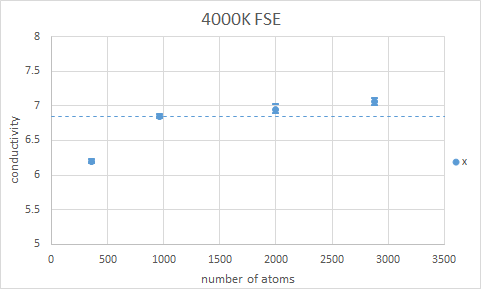
\includegraphics[width=\linewidth]{Figures/gk_fse_4K_draft.png}
\caption[gk fse 4k]{}
\label{fig:gk_fse_4K}
\end{figure}
~
\begin{figure}[h!]
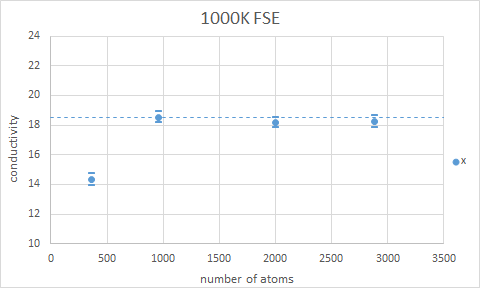
\includegraphics[width=\linewidth]{Figures/gk_fse_1K_draft.png}
\caption[gk fse 1k]{}
\label{fig:gk_fse_1K}
\end{figure}


%
\pagebreak
%


!!! MOVE TO APPENDIX? - The following lists of simulations were performed to obtain the results displayed in the 1000~K and 4000~K finite-size effect plots.

\begin{table}[h]

\centering
\caption[CONTENTS1]{4000~K}%\vspace{2mm}

\begin{tabular}{cccrr}
Supercell                        & Simulation length & \# initial conditions & \multicolumn{2}{c}{Total run time}           \\ \hline
3x3x2                             & 10 ns                     & 20                             & \multicolumn{2}{r}{2 $\mu$s}   \\ \hline
4x4x3                             & 10 ns                     & 30                             & \multicolumn{2}{r}{3 $\mu$s}               \\ \hline
\multirow{2}{*}{5x5x4} & 5 ns                       & 20                             & 1 $\mu$s     & \multirow{2}{*}{1.7 $\mu$s} \\
                                       & 1 ns                       & 70                              & 0.7 $\mu$s &                               \\ \hline
6x6x4                            & 1 ns                       & 80                              & \multicolumn{2}{r}{0.8 $\mu$s}            
\end{tabular}

%\\ \vspace{2mm}
% UNDERTABLE TEXT CAN GO HERE
\label{tab:gk_fse_times_4K}
\end{table}


%---


\begin{table}[h]

\centering
\caption[CONTENTS2]{1000~K}%\vspace{2mm}

\begin{tabular}{cccc}
Supercell                        & Simulation length & \# initial conditions    & Total run time           \\ \hline
3x3x2                             & 1 ns                        & 20                                & 0.2 $\mu$s               \\ \hline
4x4x3                             & 1 ns                        & 50                                & 0.5 $\mu$s               \\ \hline
5x5x4                             & 1 ns                        & 50                                & 0.5 $\mu$s               \\ \hline
6x6x4                             & 1 ns                        & 50                                & 0.5 $\mu$s            
\end{tabular}

%\\ \vspace{2mm}
% UNDERTABLE TEXT CAN GO HERE
\label{tab:gk_fse_times_1K}

\end{table}





%-----------------------------------------------------------
\section{\label{sec:3.Summary}Summary}
%-----------------------------------------------------------

!!! STITCH METHODS TOGETHER IN THIS SECTION. COMPARE AND CONTRAST. PROBLEMS? HOW TO APPLY THIS GOING FORWARD?

!!! EDIT ALL THIS

For bridgmanite (at conditions representing the lower mantle), we show that use of the direct method for calculation of thermal conductivity will lead to an overestimate if the simulation cell is too long (\textgreater 16 unit cells, 4000 ONLY!!!). Small cross-sectional areas (\textless 2x2 unit cells) also overestimate the thermal conductivity. This informs future work using Density Functional Theory, and will allow a model of lower mantle conductivity considering composition to be established [[[OOPS]]].

(ASSUMING THE RESULTS ARE CORRECT AND AGREE WITH GK) We see the non-linear region as described by \citet{Sellan2010} for the cell length of 6 unit cells at 1000~K, which has individually higher conductivity than expected from the linear fit through data points corresponding to lengths of 8-16 unit cells. When included in the extrapolation, this reduces the gradient of the fit, raising the intercept and thus causing conductivity to be underestimated. At temperature of 4000~K, the 6 length cell is inline with the fit through other cells with length less than 16 unit cells. As the ratio of cell length to phonon MFP increases with temperature, we believe the onset of divergence as described by Sellan et al. moves to the right (??? - MENTION ACTUAL EFFECT - QUANTIFY RATHER THAN REFERENCING GRAPH). A shorter MFP needs shorter cell lengths to display divergent conductivity, of which we have not sampled (at high temperature). DOING THE DIRECT METHOD WITH CELLS OF LENGTH LESS THAN 6 UNIT CELLS AT ANY TEMPERATURE IS A BAD IDEA BECAUSE ... 

We find conductivity is definitely dependent on CSA, but we were not able to increase CSA enough to eliminate aspect ratio-dependent divergence as reported by \citet{Hu2011}. This does support our conclusion ignoring long cell lengths however, in order to keep the aspect ratio within a reasonable limit and ensure a linear fit is extrapolated. (EVEN THOUGH 48x8x8 HAS A SMALLER RATIO than 8x2x2?)

(WAFFLE ALERT) Ignoring the specifics of this study, we stress the importance of performing finite-size analysis when performing direct method calculations.  Direct method cells spanning a range of lengths must be considered to find the linear regime for extrapolation. Cross-sectional area must be increased until the conductivity result converges. The same can be said about the Green--Kubo method, where the result converges with increasing volume. These effects vary with phonon mean-free path, sensitive to pressure, temperature, and compositional variations such as impurities. Completing finite-size effect analysis at conditions with the largest phonon mean-free path / thermal conductivity ensure all other conditions represent converged results. We believe classical molecular dynamics with interatomic potentials to be an excellent way of quantifying these effects quickly, performing ab initio methods (SHOULD I TAKE THIS SENTENCE OUT, NO PROOF OF THIS CLAIM).
